\chapter{Hyper-parameters Tuning}
\label{ch:Hyper-parameters-Tuning}

\section{Introduction}
In deep learning, hyperparameter tuning or optimization is an iterative process of searching a set of optimal values of hyperparameters to minimize the loss of the model training. Hyperparameters are the parameters that implicitly govern the learning process by controlling the training parameters' weight and bias. Unlike training parameters, hyperparameters are not trained during the learning process, but they are predefined manually by empirical data. 

However, there are few approaches for hyperparameters optimization such as trial \& error, grid search, random search, and Bayesian optimization. Such an approach finds the set of hyperparameters that yields modal optimality and minimizes the loss function. The optimization of hyperparameter is a highly iterative process that is constrained by time consumption, the number of training data available, system requirements, and available resources.  
  

\begin{figure}
    \centering
    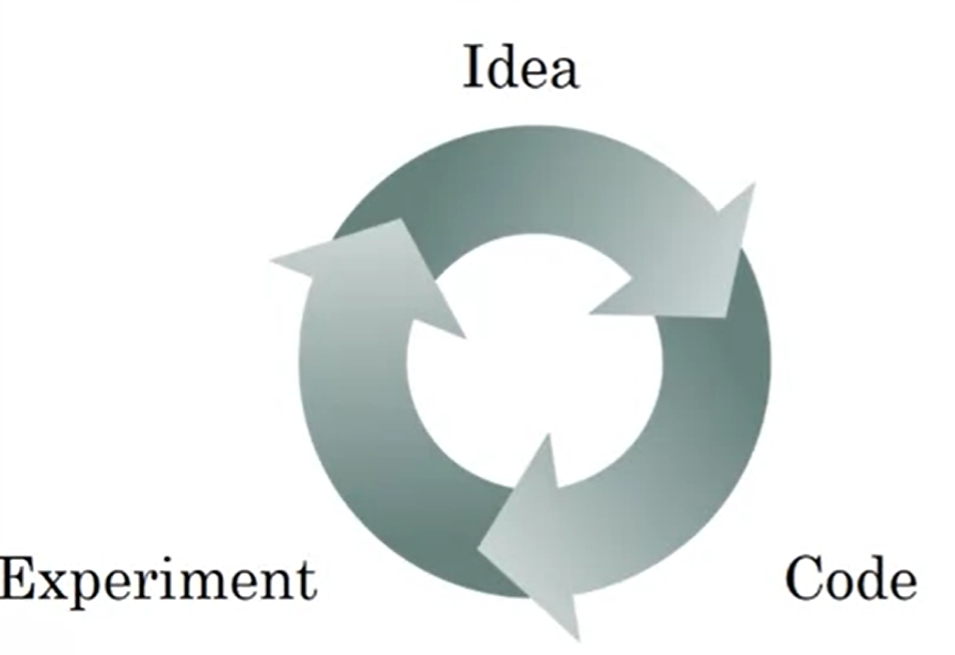
\includegraphics[width=0.45\textwidth]{Images/hypertuning.png}
    \caption{Loop of Hyperparameter Tuning Process \cite{coursera1}}
    \label{hypertuning}
\end{figure} 

\section{Approaches for Tuning Hyperparameters} 
All four approaches are briefly explained as follows. 

\subsection{Trial \& Error}
This approach is completely manual in which any value of hyperparameter is either selected by random guess or based on empirical results. If the selected values do not considerably minimize the training and testing loss, another value will be guessed based on the empirical relation between the corresponding hyperparameter and loss function. Such an approach is generally adopted by students and researchers because of the limited availability of industry-standard equipment to perform complex and time-consuming experiments. The iterative loop of this approach is pictured in Fig. \ref{hypertuning}. As per the loop, firstly the best guess for the hyperparameters is made, implement and finally assess the results and reiterate the process until the results are not convincing.

\subsection{Grid Search}
It is a naive approach to try out every possible composition of hyperparameters. Initially, the $n$ dimension grid is defined, where the $n$ dimension equals the number of hyperparameters that need to be tuned. For each dimension, define all possible values that need to have experimented with, perform training on all possible configurations and repeat until the best match is established. This technique consumes a tremendous amount of time if the size of the grid is large. However, the time consumption can be reduced if multiple computational resources are available. Usually, it is adopted when the dimension of the grid is less than or equal to 4, and as the dimension increases the time complexity increase exponentially.

\subsection{Random Search}
The main difference in this approach is the point is picked up randomly from configuration space. The graphical representation of the comparison between grid search and random search is shown in Fig. \ref{gridrandsearch}. From the above illustration, it is noticed that grid search uses only $3$ values parallelly. Whereas, the random search evaluates total $9$ models using $9$ different values. The hyperparameters space exploration is wider in the random search than the grid search which helps find the best values in a lower number of iteration. Therefore, it is used when configuration space has high dimensionality.  

\begin{figure}
    \centering
    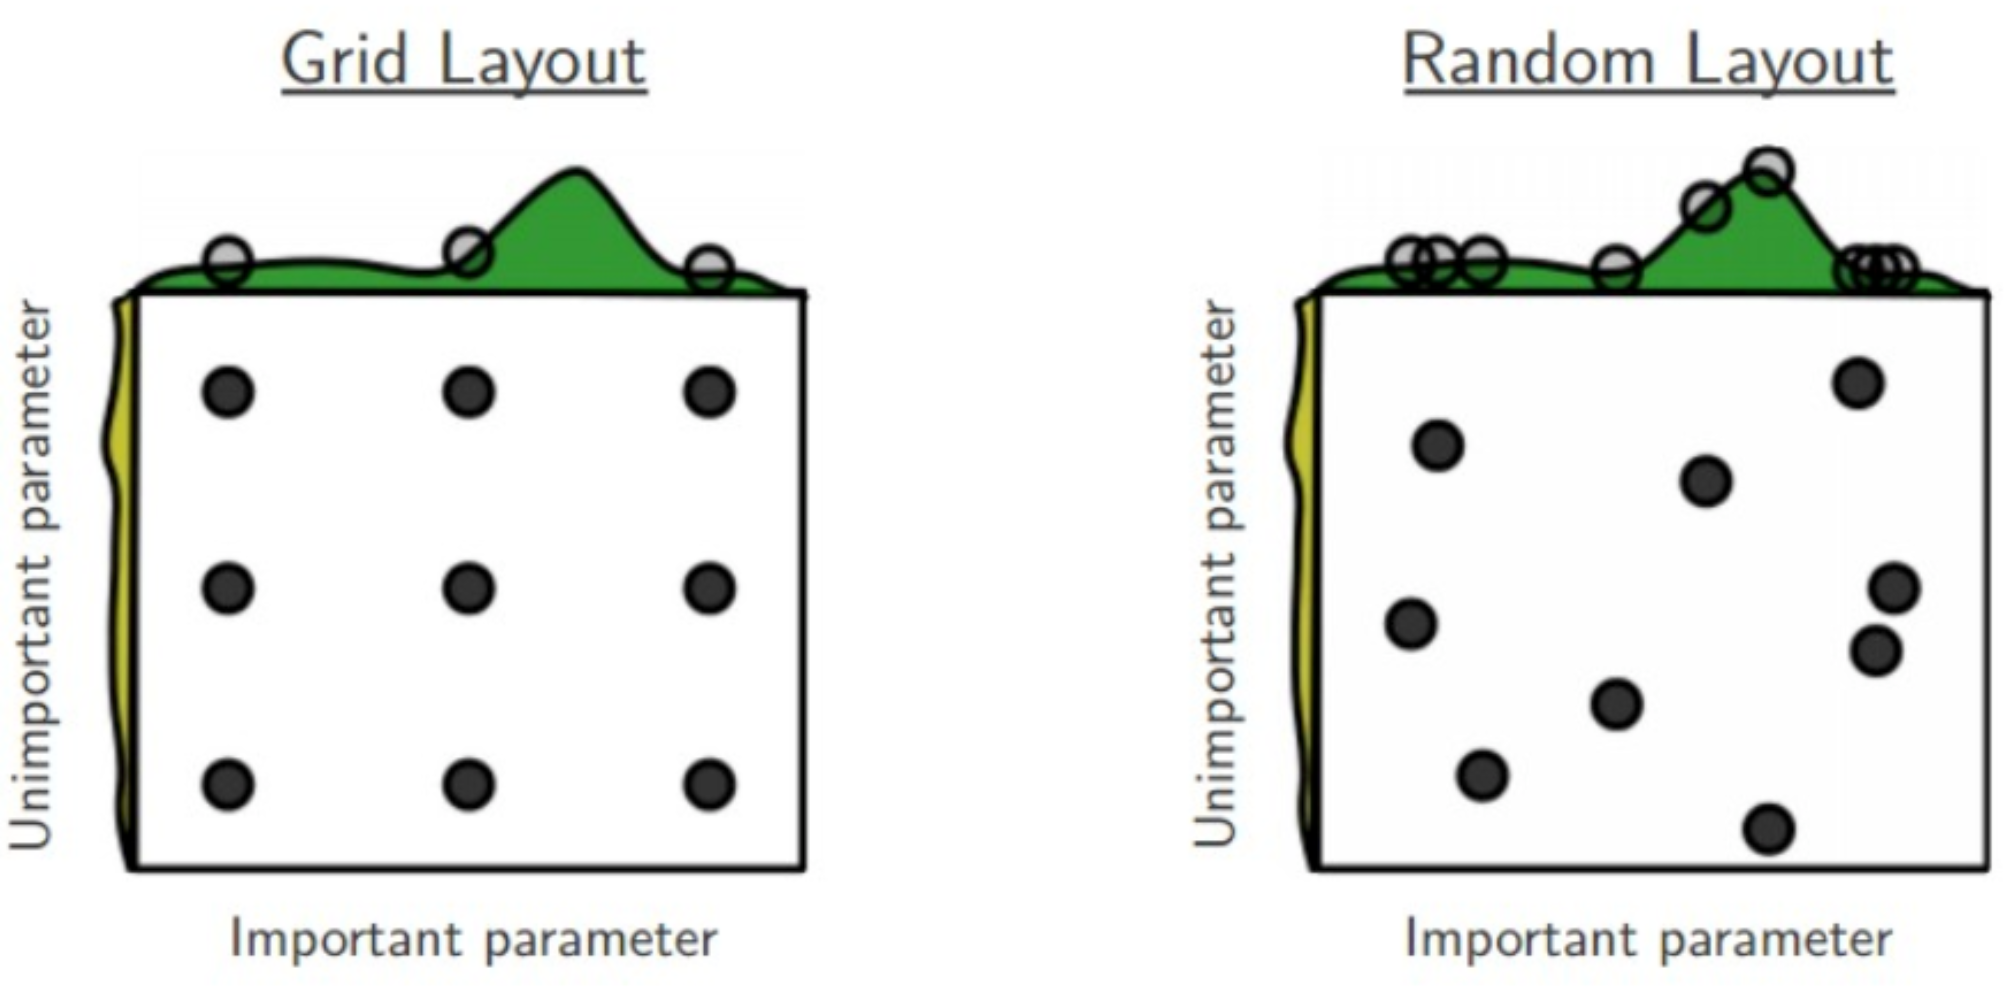
\includegraphics[width=0.8\textwidth]{Images/gridrandsearch.png}
    \caption{Configuration Space Layout of Grid Search and Random Search Approaches \cite{Bergstra}}
    \label{gridrandsearch}
\end{figure}

\subsection{Bayesian Optimization}

\begin{figure}
    \centering
    \begin{subfigure}[]
        \centering
        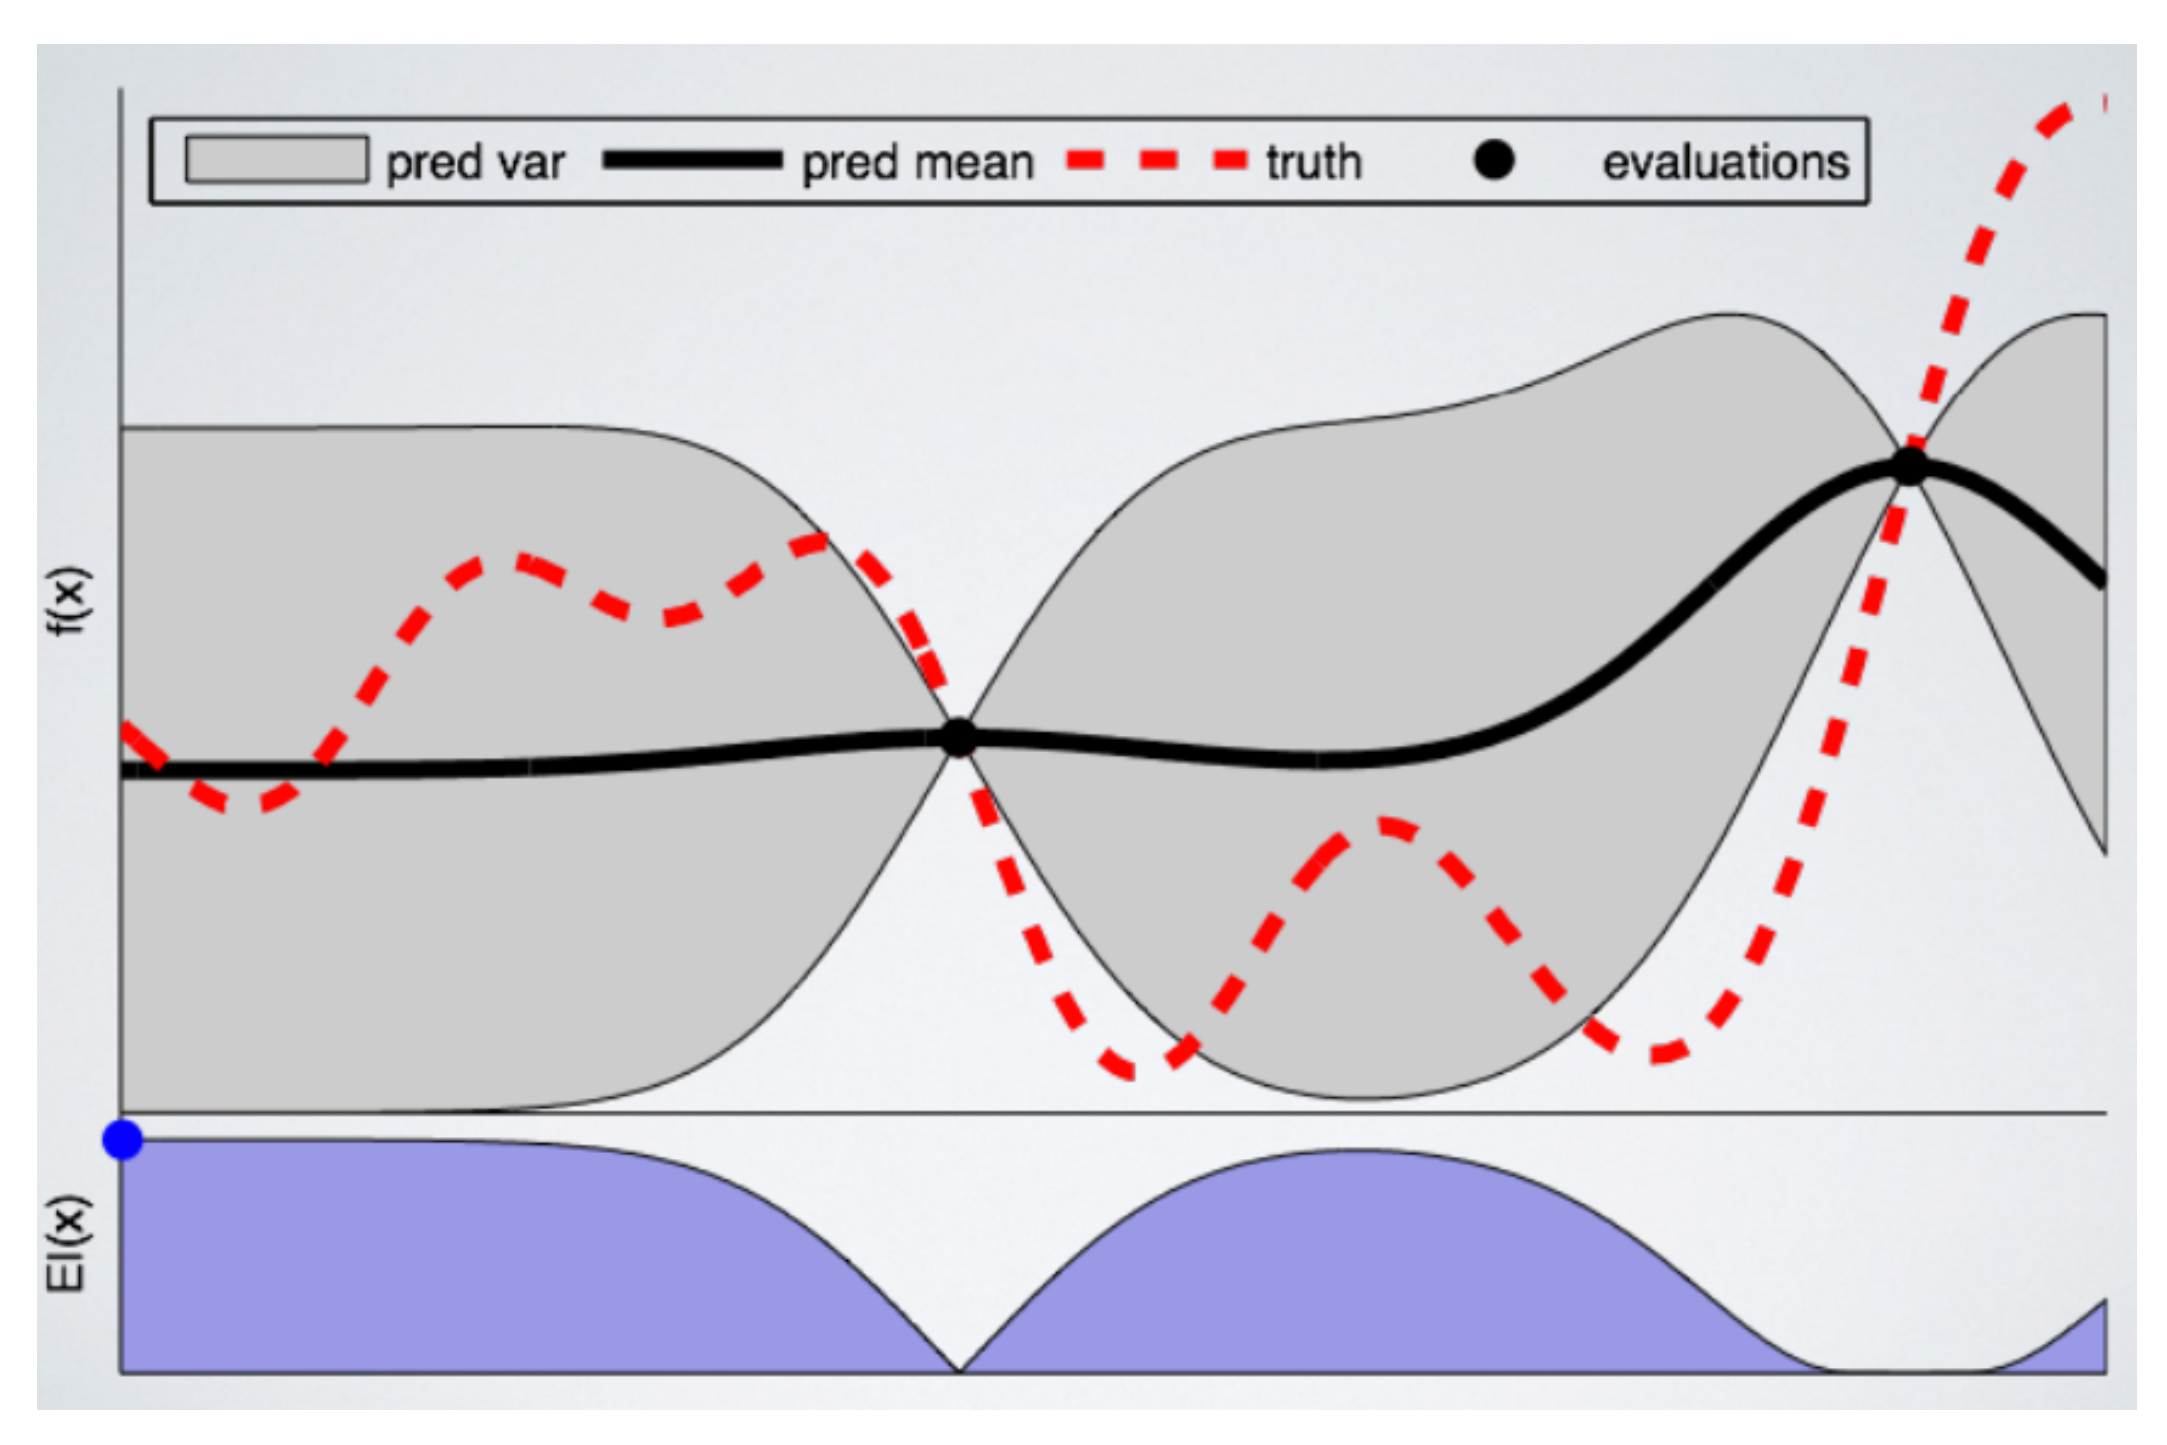
\includegraphics[width=0.9\textwidth]{Images/2point.png}
    \end{subfigure}
    \begin{subfigure}[]
        \centering
        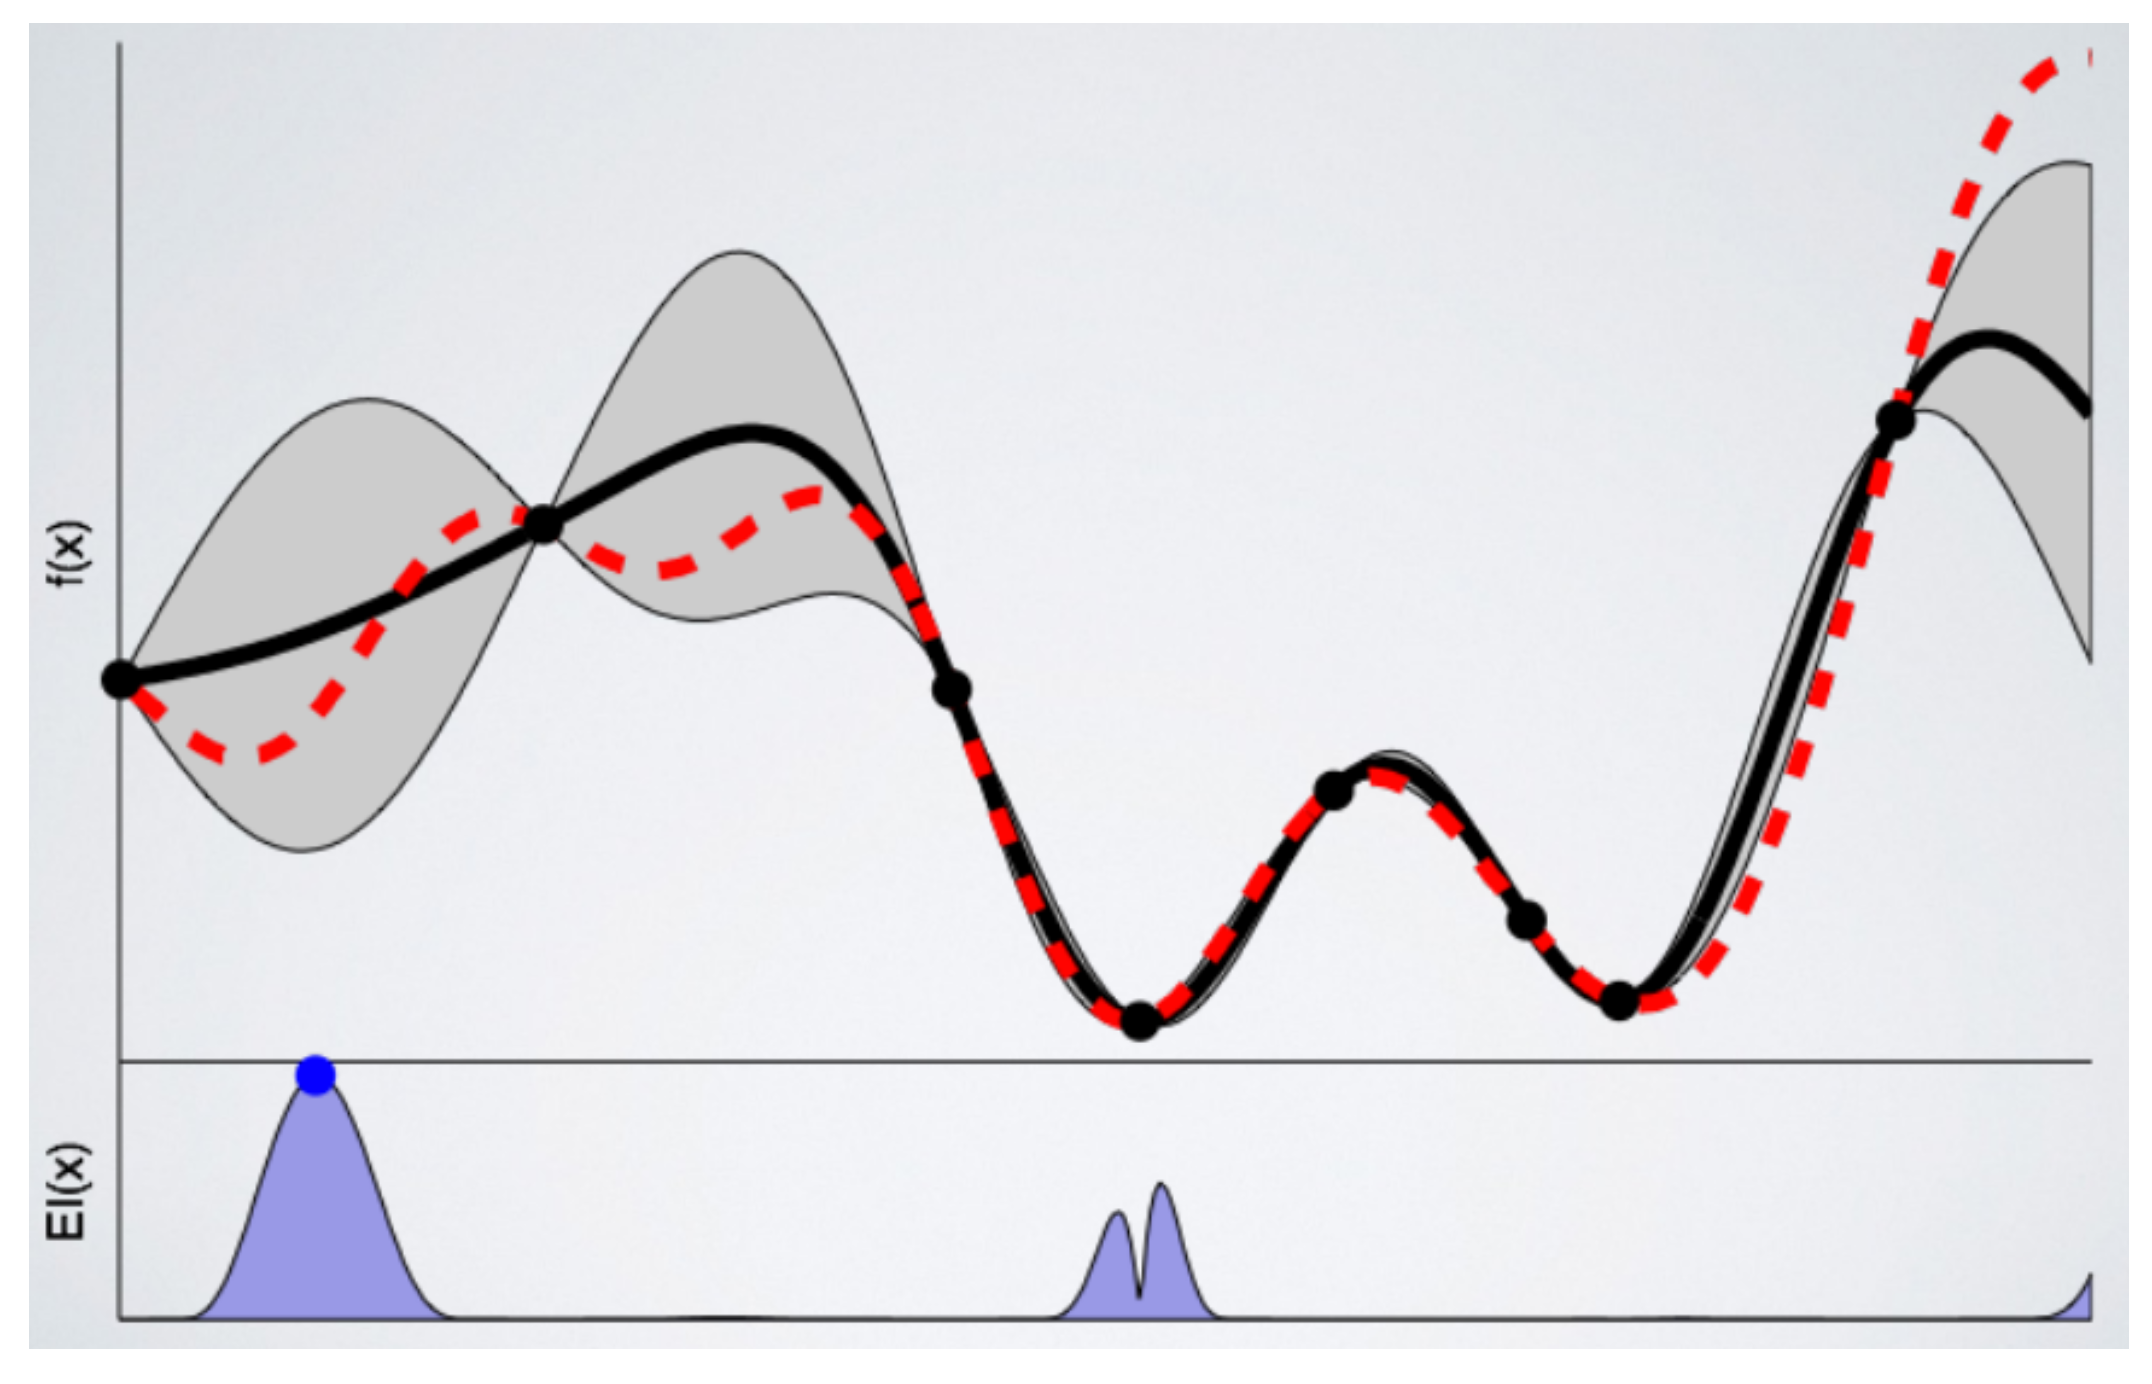
\includegraphics[width=0.9\textwidth]{Images/8point.png}
    \end{subfigure}
    \caption{Bayesian Optimization Process for (a) $2$ Trained Model, and (b) $8$ Trained Models \cite{Bayesianoptimization}}
    \label{bayesianoptimization}
\end{figure} 

This is an autonomous approach that adept the configuration space of hyperparameters at each iteration based on model evaluation from the last iteration. At each iteration, the surrogate model becomes more and more confident that yields the minimum training loss. The Gaussian process is used as the surrogate to predict the mapping from hyperparameter configuration to the region of interest, additionally, it also derives the range of uncertainty of weight and bias. The Bayesian optimization process after $3$ and $8$ model evaluation are shown in Fig. \ref{bayesianoptimization}(a) and Fig. \ref{bayesianoptimization}(b) respectively. The uncertainty is high in the areas where little information available. After each model evaluation, it adapts the new point (blue dot) on which the training will perform. As the number of trained models increases, the confidence of the surrogate will surge. However, this approach is only used for numerical hyperparameter, and it is impossible to stop earlier if the training progress is poor.  

\begin{figure}
    \centering
    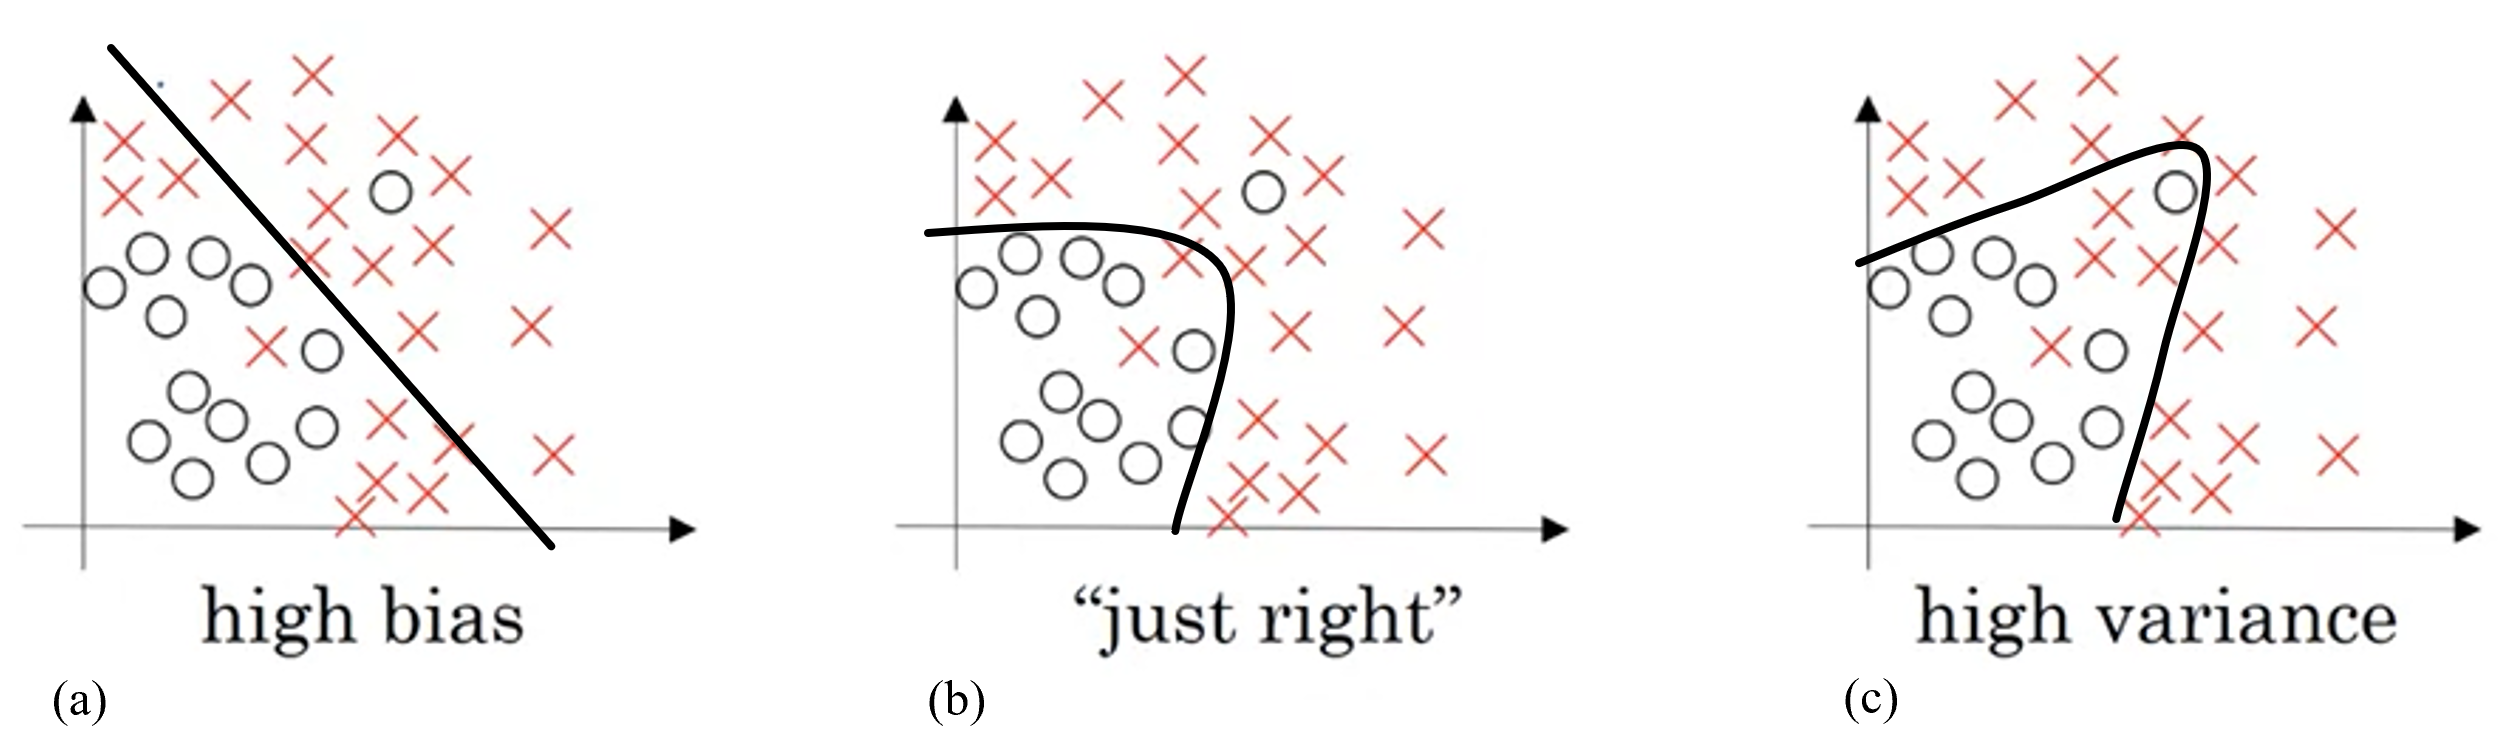
\includegraphics[width=0.9\textwidth]{Images/tradeoff.png}
    \caption{Classifier Behaviour for Various Bias and Variance Conditions\cite{coursera1}}
    \label{tradeoff}
\end{figure}

\section{Bias and Variance Trade-off}
Bias and Variance are the main sources of an estimation or prediction error. Bias is the error due to deviation of estimation from the true value of a parameter, on the other hand, variance is the error due to deviation of measurement from expectation. In other words in the context of deep learning, the bias is the error due to the difference between training error and ideal error (usually $0\%$). And the variance is the error due to the difference between testing and training accuracy. For instance, the bias will dominate the error if the training error is large, on the flip side the variance will be big if the difference between training and testing error is large as mentioned in table \ref{biasvariance}. In the third case, if the training error is high and the testing error is even worst, the trained model has both high variance and high bias. A simple classifier's behavior is shown in Fig. \ref{tradeoff}. The highly linear classifier in Fig. \ref{tradeoff} (a) has a high bias that under-fits the data, whereas the highly non-linear classifier in Fig. \ref{tradeoff} (c) has a high variance that over-fits the data. However, the classifier in Fig. \ref{tradeoff} (b) is reasonably fit to the data and it has just the right characteristic of non-linearity that prevents it from over-fitting.             

\begin{table}
    \centering
    \begin{tabular}{|c|c|c|}
        \hline
        Training Error & Testing Error & Remarks \\
        \hline
        1 \% & 11 \% & High Variance \\
        \hline
        15 \% & 16 \% & High Bias \\
        \hline
        15 \% & 30 \% & High Variance \& Bias \\
        \hline
        0.5 \% & 1 \% & Low Variance \& Bias \\
        \hline        
    \end{tabular}
    \caption{Effect of Variation in Train and Test Error on Bias and Variance}
    \label{biasvariance}
\end{table}

\begin{figure}
    \centering
    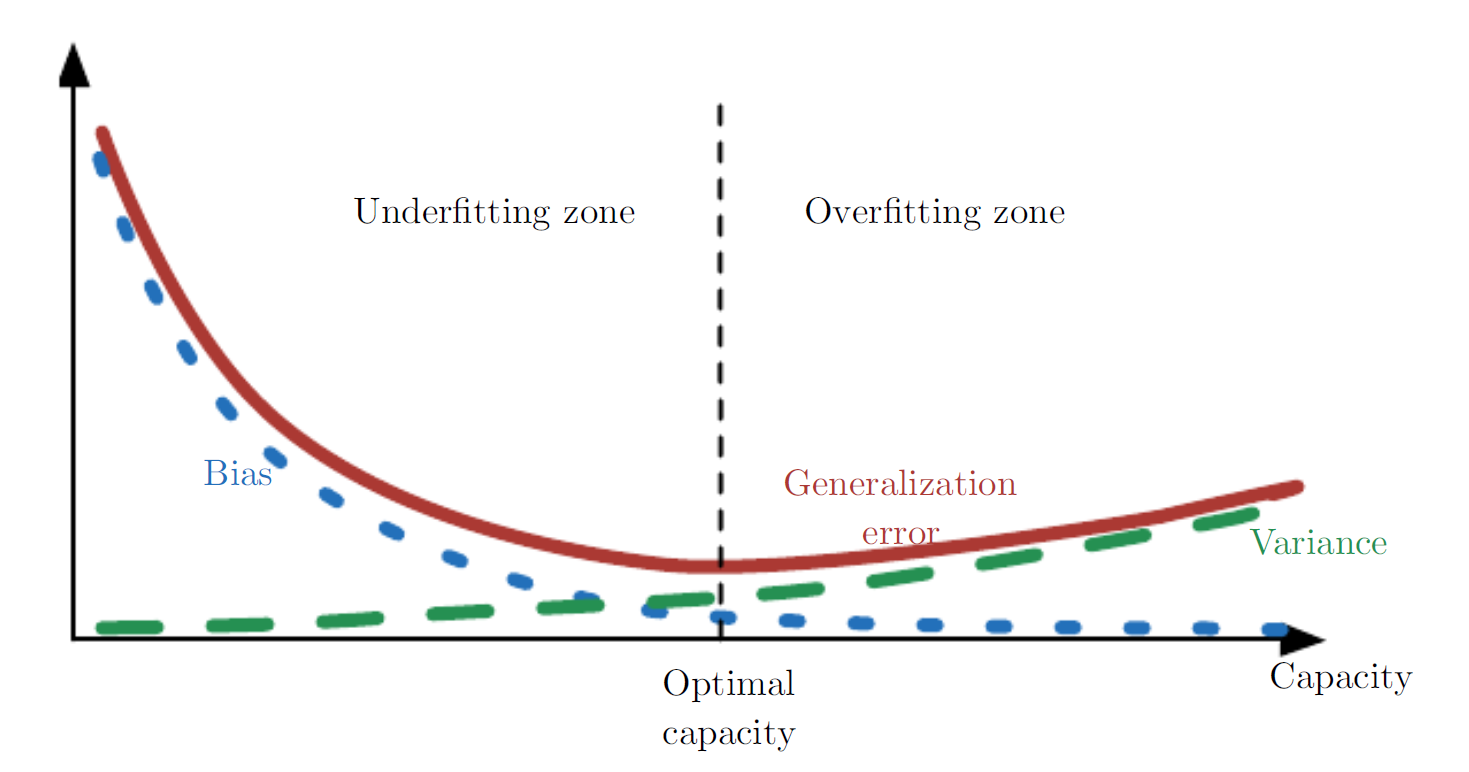
\includegraphics[width=0.7\textwidth]{Images/relationship.png}
    \caption{Relationship between Bias and Variance \cite{goodfellow}}
    \label{relationship}
\end{figure}

The bias and variance are tightly connected and they are inversely proportional to each other as seen in Fig. \ref{relationship}. As per the illustration, the meaning of increase the capacity of the model is to reduce the bias and rise the variance. As the capacity is gradually rising, the model training moves from the under-fitting region to an optimal point where the generalized error is optimum. The capacity of a model can be increase by using a deeper network by adding more layers, as result, the overall bias is considerably diminished. On the contrary, the model variance can be narrow down by using the larger dataset and use a similar source for train and test data which efficiently lessens the variance without affecting the bias.      

\section{List of Tunable Hyperparameters}
There is a list of tunable hyperparameters that use to regularize the deep learning model; however, we only discuss the hyperparameters that are used in this study in the following subsections.  

\subsection{L2 Regularization}
By regularization means to prevent the model from overfitting the data. For the object detection application in deep learning, there is a small amount of training dataset available based on the capacity (size) of a neural network. Therefore, over-fitting of a network is a common problem in object detection. Such a problem can be used by regularizing the neural network. 

Particularly, in the L2 regularization, the weight metric is penalized by the definition of L2 regularization parameter $(\lambda)$. In the definition of the loss function, the additional term added that known as Frobenius norm or second norm as written in Eq. (\ref{L2regularization}). By choosing a bigger value of $\lambda$ prevents over-fitting, but selecting higher than the required value tends to increase the bias and results in under-fitting, hence the L2 regularization parameter needs to be tuned to prevent from over-fitting consequently taking care of bias.   

\begin{equation}
\label{L2regularization}
J(w, b)=\frac{1}{m} \sum_{i=1}^{m} L\left(a^{(i)}, y\right)+\frac{\lambda}{2 m}\|w\|_{2}^{2}
\end{equation}

Where, $\|w\|_{2}^{2}=\sum_{j=1}^{n_{x}} w_{j}^{2}=w^{T} \cdot w$, $\lambda$ is a regularization parameter, J is a cost function, a is an activation from corresponding layer, m is the number of training data, L is a loss function, y is a true or desire output from ground truth data, and i is an iteration index.  

\begin{equation}
\begin{aligned}
\label{weightdecay}
\omega^{[l]} &= \omega^{[l]}-\alpha\left[(\text{from back-prop})+\frac{\lambda}{m} w^{[l]}\right] \\
&=\omega^{[l]}-\frac{\alpha \lambda}{m} \cdot \omega^{[l]}-\alpha(\text {back-prop}) \\
&= [1 - \frac{\alpha \lambda}{m}] \cdot \omega^{[l]} -\alpha(\text {back-prop})
\end{aligned}
\end{equation}

The primary intuition behind L2 regularization is explained by Eq.(\ref{weightdecay}). By using regularization, the update step for weight metric in forward propagation is modified as seen in Eq.(\ref{weightdecay}). From this equation, it has been seen that the weight metric is decay by a factor of $\frac{\alpha \lambda}{m}$, thus L2 regularization is also called weight decay.

\subsection{Data Augmentation}
Data augmentation is a method to improve network accuracy by randomly transforming the training data. Before training, the training dataset is pass through the data augmentation function to generate random transformations such as adding color jitter in HSV color space, flipping horizontally, and randomly scaling up to 10 or 10$\%$ as shown in Fig. \ref{augmentation}. It is another way of increasing the training dataset.

\begin{figure}
    \centering
    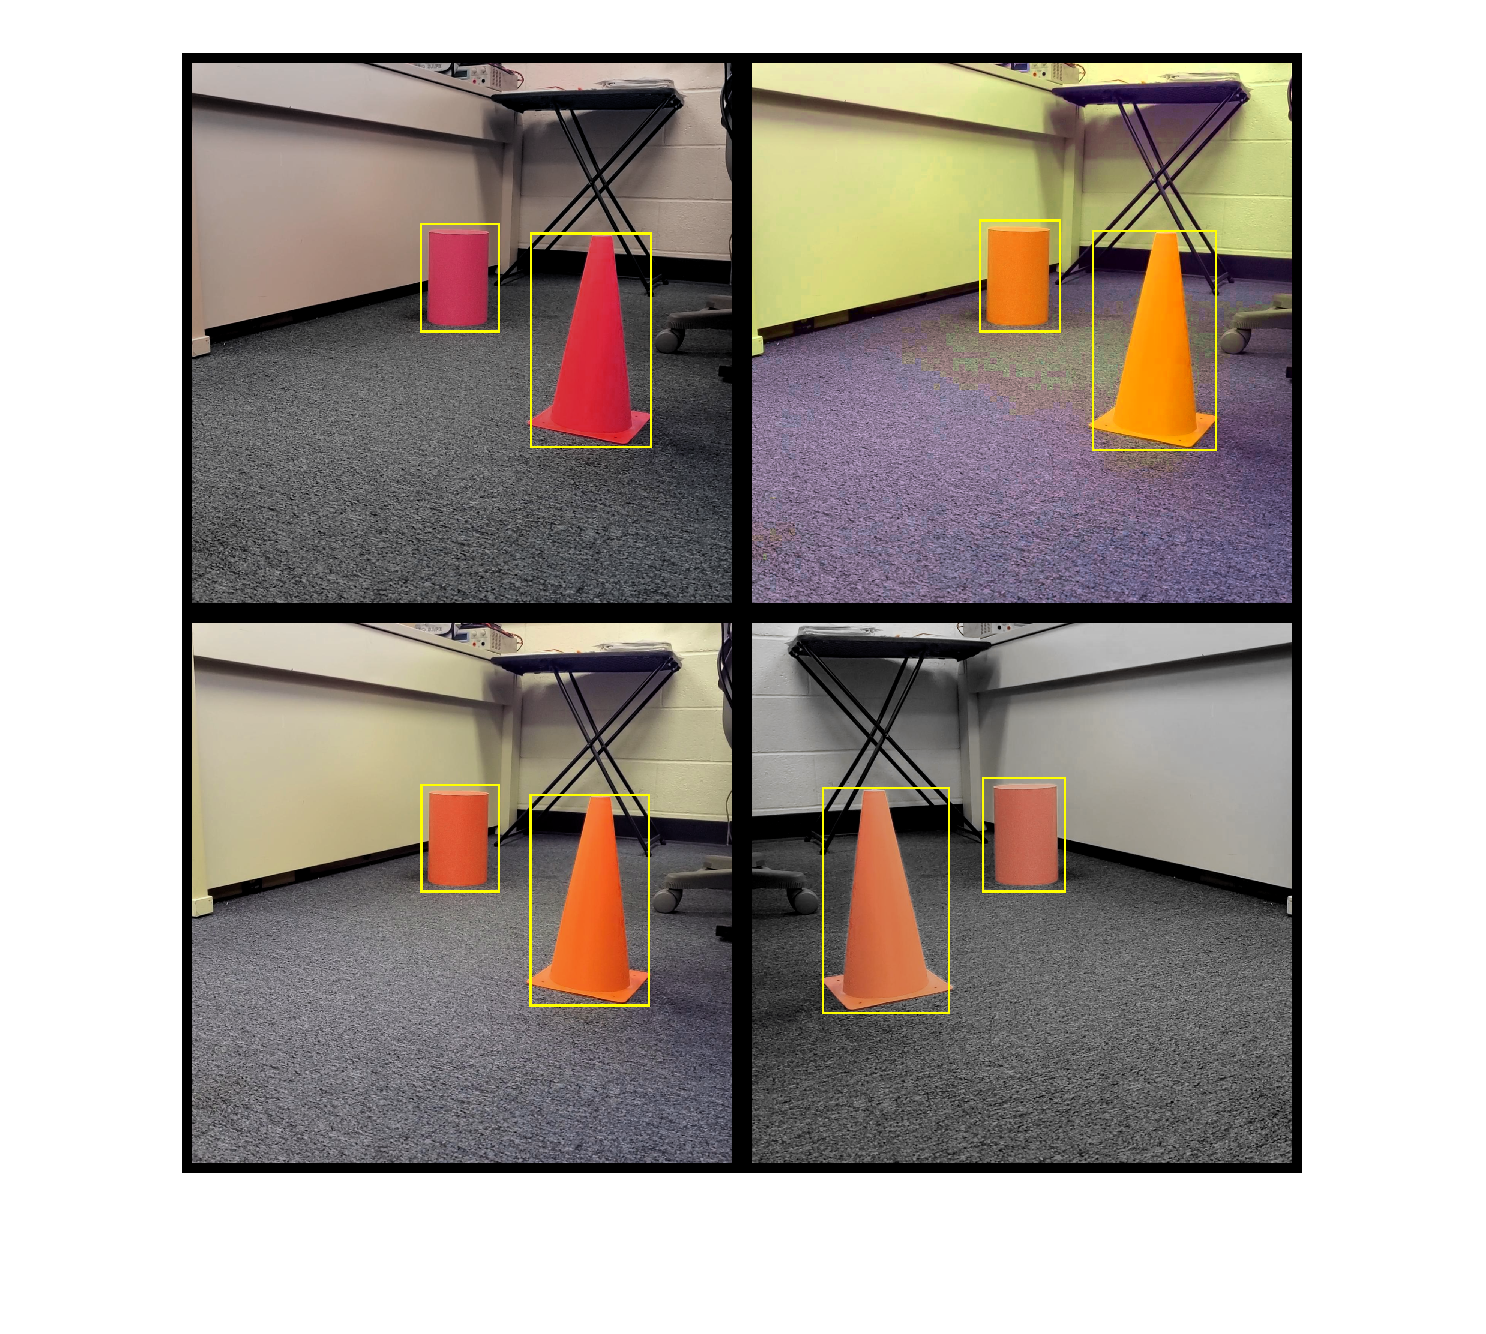
\includegraphics[width=0.7\textwidth]{Images/augmentation.png}
    \caption{Training Data Augmentation}
    \label{augmentation}
\end{figure}

\subsection{Mini-batch Size}
In deep learning, the size of the dataset is usually large, thus a single iteration in training takes a lot of time. Instead, the training data is divided into small sizes of mini-batches. By transforming training data into mini-batches to train the network, the speed is quite faster than the complete batch of data. However, the number of training examples per mini-batch is a decisive factor in training accuracy. The small mini-batch size is extremely noisy since new data is passed at each iteration. On contrary, the large mini-batch size is extremely slow in convergence. Therefore, the mini-batch size is selected in a way that the learning progresses with enough speed and a considerable amount of noise.  

\subsection{Number of Epoch}
The number of an epoch is a hyperparameter that defines the number of times the training algorithm passes through the complete dataset. Each epoch states the training batch has a chance to improve the internal training parameter. Traditionally, the number of epoch should be large enough that allows an algorithm to run until sufficient accuracy is achieved.

\subsection{Momentum}
The momentum parameter is used in the gradient descent algorithm to speed up the process by utilizing the moving average. The velocity in the training process is defined in Eq.(\ref{momentum}), which is an exponentially weighted average of last n velocities where n is the number of samples considers in evaluating average at each iteration. The value of the momentum parameter ($\beta$) is carefully selected by which the sequential plot of weighted average fits on noisy data. In Fig.\ref{momentumpara}, the behavior of exponentially weighted average for different value of momentum parameter is illustrated. Since the lower value of $\beta$ averages a lesser number of samples, the plot for $\beta = 5$ is much noisy.     

\begin{equation}
\label{momentum}
V_{t}=\beta V_{t-1}+(1-\beta) S_{t}
\end{equation}

\begin{figure}
    \centering
    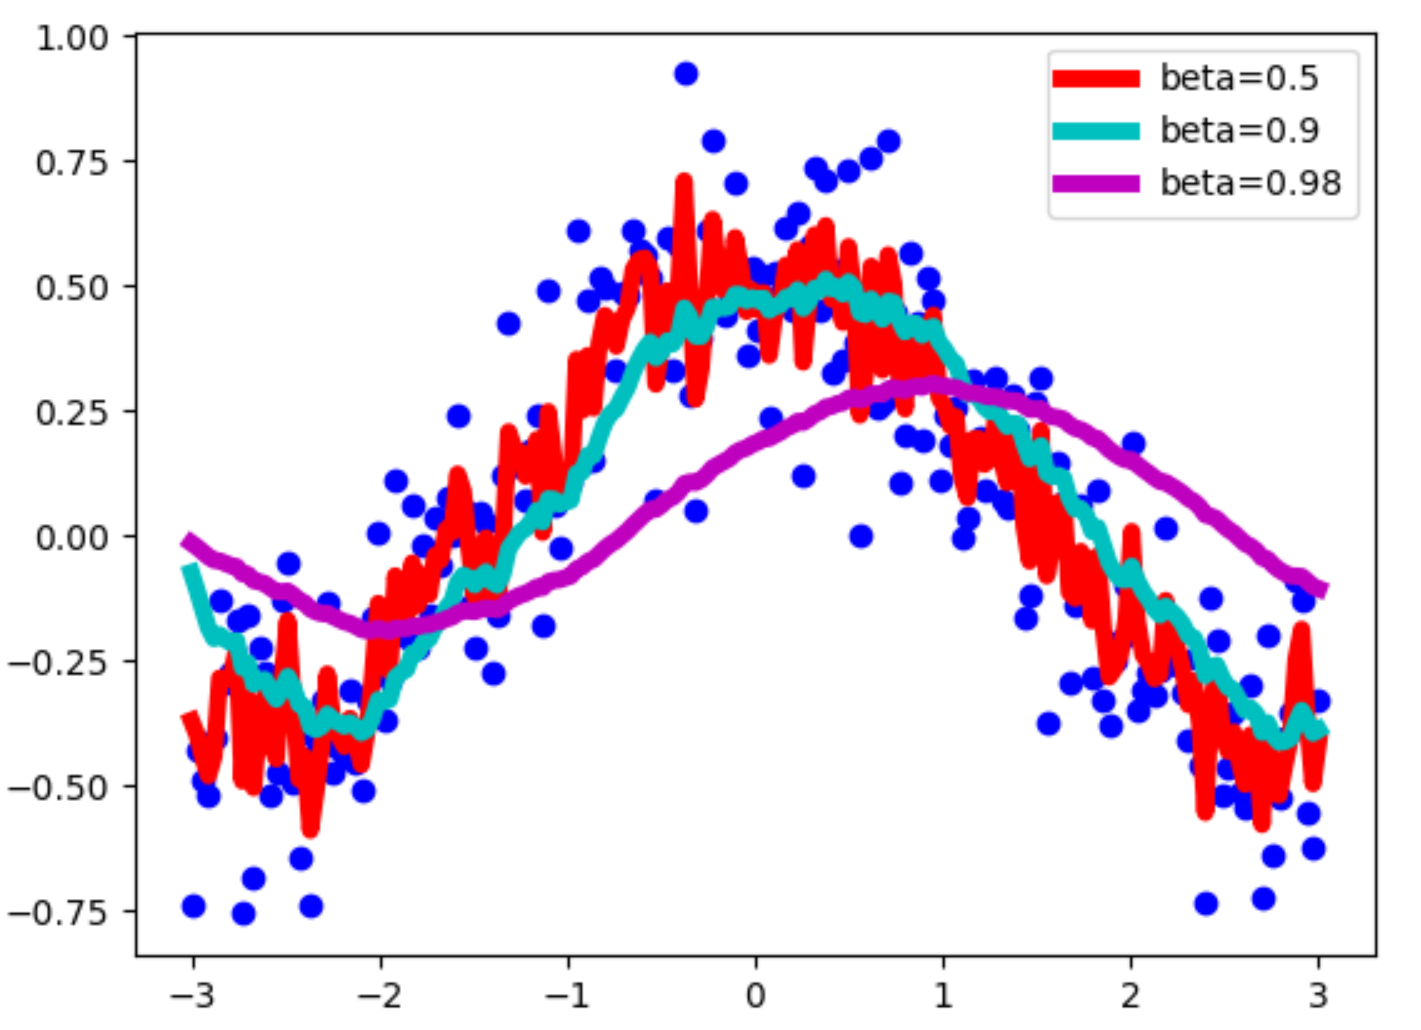
\includegraphics[width=0.6\textwidth]{Images/momentumpara.png}
    \caption{Exponentially Weighted Averages for Different Values of $\beta$ \cite{gradientdescent}}
    \label{momentumpara}
\end{figure}

\subsection{Learning Rate}
Learning rate is a hyperparameter that represents the step size of the gradient in direction of convergence. This is an important parameter in training because the accuracy in training is greatly dependant on the amount learning rate. Usually, the learning rate is selected to be 0.001 for training small to medium size neural network, however, if the large size network needs to training on a complex dataset, the variation in learning rate is adopted as the training progresses. There are few approaches used to decay the learning rate online. One of them is discrete step decay, in which the larger value is selected initially and is reduced at every predefined number of iterations.            


